\documentclass[a4paper,twoside]{article}

\usepackage{epsfig}
\usepackage{subfigure}
\usepackage{calc}
\usepackage{amssymb}
\usepackage{amstext}
\usepackage{amsmath}
\usepackage{amsthm}
\usepackage{multicol}
\usepackage{pslatex}
\usepackage{subfigure}

\usepackage{apalike}
\usepackage{SCITEPRESS}     % Please add other packages that you may need BEFORE the SCITEPRESS.sty package.

\subfigtopskip=0pt
\subfigcapskip=0pt
\subfigbottomskip=0pt

\begin{document}

\title{EvoloPy: An open source Nature-Inspired Optimization Toolbox in Python}

\author{\authorname{First Author Name\sup{1}, Second Author Name\sup{1} and Third Author Name\sup{2}}
\affiliation{\sup{1}Institute of Problem Solving, XYZ University, My Street, MyTown, MyCountry}
\affiliation{\sup{2}Department of Computing, Main University, MySecondTown, MyCountry}
\email{\{f\_author, s\_author\}@ips.xyz.edu, t\_author@dc.mu.edu}
}

\keywords{The paper must have at least one keyword. The text must be set to 9-point font size and without the use of bold or italic font style. For more than one keyword, please use a comma as a separator. Keywords must be titlecased.}

\abstract{EvoloPy is an open source and cross-platform Python toolbox that implements a wide range of classical and recent nature-inspired metaheuristic algorithms. The goal of this toolbox is to facilitate the use of metaheuristic algorithms by non-specialists coming from different domains. With a simple interface and minimal dependencies, it is easier for researchers and practitioners to utilize EvoloPy for optimizing and benchmarking their own defined problems using the most powerful metaheuristic optimizers in the literature. On the other hand, the design of this toolbox makes it very easy for the researchers in the domain to integrate their own optimizers and compare their performance to the state of art algorithms. }


\onecolumn \maketitle \normalsize \vfil
\section{\uppercase{Introduction}}

\label{sec:introduction}


Nature-inspired algorithms are population based metaheuristics which are inspired by different natural phenomena and designed for solving and optimizing complex problems. Due to their stochastic and non-deterministic nature, there have been a growing interest in ivestigating their applications for solving complex problems when the search space is extremely large and it is impossible to solve them with conventional search methods \cite{Yang_2013}. 

In general, nature-inspired algorithms can fall into two main categories: Swarm Intelligent algorithms and Evolutionary Algorithms. Swarm intelligence algorithms simulate the natural swarms such as flocks of birds, ant colonies, and schools of fishes. Popular algorithms fall in this category are Particle Swarm Optimization (PSO) \cite{Kennedy95}, and Ant Colony Optimization (ACO) \cite{Koro_ec_2009}. More recent Swarm intelligence algorithms include Cuckoo Search (CS) \cite{Yang2009}, Grey Wolf Optimizer (GWO) \cite{Mirjalili201446}, Multi-Verse Optimizer (MVO) \cite{Mirjalili2016}, Moth-flame optimization (MFO) \cite{Mirjalili2015228}, Whale Optimization Algorithm (WOA) \cite{Mirjalili201651}, Bat Algorithm (BAT) \cite{Yang2010}, Firfly Algorithm (FFA) \cite{Yang2010FFA}, and many others. Most of Swarm intelligence algorithms reach the best solution by exchanging the information between the swarm's individuals. 

On the other hand, evolutionary based algorithms are inspired by some concepts from the Darwinian theories about evolution and natural selection. Such algorithms include Genetic algorithm (GA) \cite{Sivanandam}, Genetic Programming (GP)\cite{Koza1992}, and Evolution Strategy (ES)\cite{Beyer2002}. These algorithms use different strategies to evolve and find good solutions for difficult problems. 

An important turn in the research field was made when the No Free Lunch Theorem (NFL) was released. NFL states that no algorithm is superior to all other algorithms in all optimization problems. This means that if an algorithm A outperforms another algorithm B for some type of optimization problems then algorithm B outperforms A in another types of problems. Since then, researcher and practitioners have been developed a wide range of metaheuristic algorithms and investigated their applications in different types of tough optimization problems. In the last decade, most of the researchers implemented and shared their proposed optimizers in Matlab. This is due its simplicity and ease of use. However, Matlab is a commercial and expensive software and portability is a big issue.

In this paper, we introduce EvoloPy which is a framework writen in Python that provides well-regarded and recent nature inspired optimizers. The goal of the package is to take the advantage of the rapidly growing scientific community of Python and provide a set of robust optimizers as free and open source software. We believe that implementing such algorithms in Python will increase their popularity and portability among researchers. Moreover, the powerful libraries and packages available in Python will make it more feasible to apply metaheurostic algorithms for solving complex problems on a much larger scale.



\section{\uppercase{Related Work}}
Today, there exist many different nature-inspired optimization libraries and toolboxes. Some of them are developed for special type of nature-inspired optimization like GEATbx \cite{GEATbx}, which is a toolbox contains many variants of the genetic algorithms, and genetic Programming. GEATbx is implemented in MATLAB environment and provides many global optimization capabilities. The authors in \cite {GAlib} developed GAlib library, which contains a set of C++ genetic algorithm tools and operators for different optimization problems. GAlib is built on UNIX platforms and supported parallel experiments. 

In \cite {DEAP_JMLR2012}, the authors developed a novel evolutionary computation python framework called DEAP to simplify the execution of many optimization ideas with  parallelisation features. The DEAP Framework includes many nature-inspired algorithms with different variations such as: Genetic Algorithm, Genetic Programing (GP), Evolution Strategies (ES), Particle Swarm Optimization (PSO), Differential Evolution (DE), and multi-objective optimization. In addition, DEAP includes Benchmarks modules containing many test functions for evaluations. In \cite{Wagner04}, the author presents a generic optimization environment named HeuristicLab, which is implemented using C\# language. HeuristicLab is a framework for heuristic, evolutionary algorithms, and machine learning. HeuristicLab includes many algorithms such as: Genetic Programming, Age-layered Population, Structure (ALPS), Evolution Strategy, Genetic Algorithm, Island Genetic Algorithm, Particle Swarm Optimization, Relevant Alleles Preserving GA, and many others. 

In \cite{Durillo2011}, jMetal is developed, which is a framework contains many metaheuristic algorithms implemented in Java programming. The authors employ the object-oriented architecture to develop the framework. jMetal includes many features such as: multi-objective algorithms, parallel algorithms, constrained problems, and different representations of the problem variables. In \cite{Cahon2004,humeau13}, the authors present a white-box object-oriented framework called ParadisEO. ParadisEO is developed by integrating Evolving Objects (EO) - which is an C++ evolutionary computation framework - and many distributed metaheuristics including local searches (LS), and hybridization mechanisms.  

Comparing our developed framework to the frameworks listed above, all frameworks were contained traditional nature-inspired algorithms such as: GA, GP, PSO, ES, and many others. Whereas in our developed framework, the framework includes the traditional nature-inspired algorithms such as PSO and nine recent nature-inspired algorithms such as: GWO, MVO, MFO, WOA, BAT, CS, and FFA. To the best of our knowledge, EvoloPy framework is the first work contains such optimizes that developed in Python language. EvoloPy is developed in very efficient way to solve computationally expensive optimization functions with very high dimensions.


\section{\uppercase{Why Python?}}

Python is a general purpose scripting language which has a clear and simple syntax. With the rapid development of mature, advanced  and open source scientific computing libraries and packages, Python became as one of the most popular and powerful languages for scientific computing.
Moreover, Python has cross-platform runability, which works with different operating systems, and has ability to access libraries written in different programming languages and computing environments. Python also can support small-form devices, embedded systems, and microcontrollers. In addition, Python needs very minimal setup procedure to start with. Python uses modular and object based programming, which is a popular methodology to organize classes, functions, and procedures into hierarchical namespaces. All these reason has turned Python to be a popular language in a huge community of scientists. 

\section{\uppercase{Toolbox Overview and Featured algorithms}}

EvoloPy provides a set of classical and recent nature-inspired metaheuristic optimizers with an easy-to-use interface. The toolbox incorporates four main components which are described as follows: 

\begin{itemize}
\item The Optimizer: this is the main interface of the of the toolbox in which the users can select a list of optimizers to run in their experiment. Using this interface, the user can configure common parameters for the algorithms like the maximum number of iterations for each run, the size of the population and the number of runs. In addition, a list of benchmark problems can be selected.

\item The metaheuristics algorithms: simply this part includes the list of implemented optimizers in the framework. At the time of writing this paper, eight algorithms are implemented. A brief description of each algorithm is given as follows:

\begin{itemize}
\item PSO
\item  FFA
\item GWO
\item WOA 
\item MVO
\item MFO
\item BAT
\item CS
\end{itemize}



\item Benchmark functions and problem definition: This part includes a set of common benchmark problems commonly used in the literature for the purpose of comparing different metaheuristic algorithms. Any new user-defined cost function could be added to this list.

\item Results management and visualization: this component is responsible about exporting the results and and storing them in one common CSV file. 
\end{itemize}


\section{\uppercase{Design issues}}

Most of nature inspired metaheuristics are population-based algorithms. These algorithms start by randomly initializing a set of individuals each of which represents a candidate solution. Conventionally, in most of state-of-art evolutionary algorithms frameworks, populations are implemented as 2-dimensional arrays while individuals are implemented as 1-dimensional array. For example an individual $I$ and a population $P$ can be represented as given in equations \ref{eq:individual} and \ref{eq:population}.

\begin{equation}
I_{i}=[\begin{array}{cccc}
x_{i}^{1} & x_{i}^{2} & ... & x_{i}^{d}\end{array}]
\label{eq:individual}
\end{equation}

\begin{equation}
P=\left[\begin{array}{cccc}
x_{1}^{1} & x_{1}^{2} & ... & x_{1}^{d}\\
x_{2}^{1} & x_{2}^{2} & ... & x_{2}^{d}\\
\vdots & \vdots & \vdots & \vdots\\
x_{n}^{1} & x_{n}^{2} & ... & x_{n}^{d}
\end{array}\right]
\label{eq:population}
\end{equation}

In EvoloPy, \texttt{Numpy} is chosen to define and represent the populations and individuals in the optimizers. \texttt{Numpy} is an open-source extension to Python that provides common scientific computing and mathematical routines as pre-compiled and fast functions. \texttt{NumPy} also supports large multidimensional arrays and matrices and it offers a variety range of functions to handle and perform common operations on these arrays. \texttt{Numpy} has many things in common with Matlab. This makes it easier for researchers who are familiar with Matlab use EvoloPy. 

The core data structure \texttt{ndarray} (abbreviation for N-dimensional array) in \texttt{Numpy} is used to define 1-dimensional and 2-dimensional arrays that represent individuals and populations, respectively. For example, to define a randomly generated initial population with 50 individuals and 100 dimensions the following python line of code can be used

\texttt{initialPop = np.random.rand(500,100)}


Moreover, with \texttt{Numpy} it is possible to perform vector operations in simple and compact syntax. For example, a common operation is used in many metaheuristic algorithms is to check the boundaries of the elements of the individuals after updating them. This can be performed all at once with \texttt{Numpy} as follows:

\texttt{newPop=numpy.clip(oldPop, lb, ub)}

Where \texttt{lb} and \texttt{ub} are the upper and lower bounds respectively.

\begin{figure*}[http]
\centerline{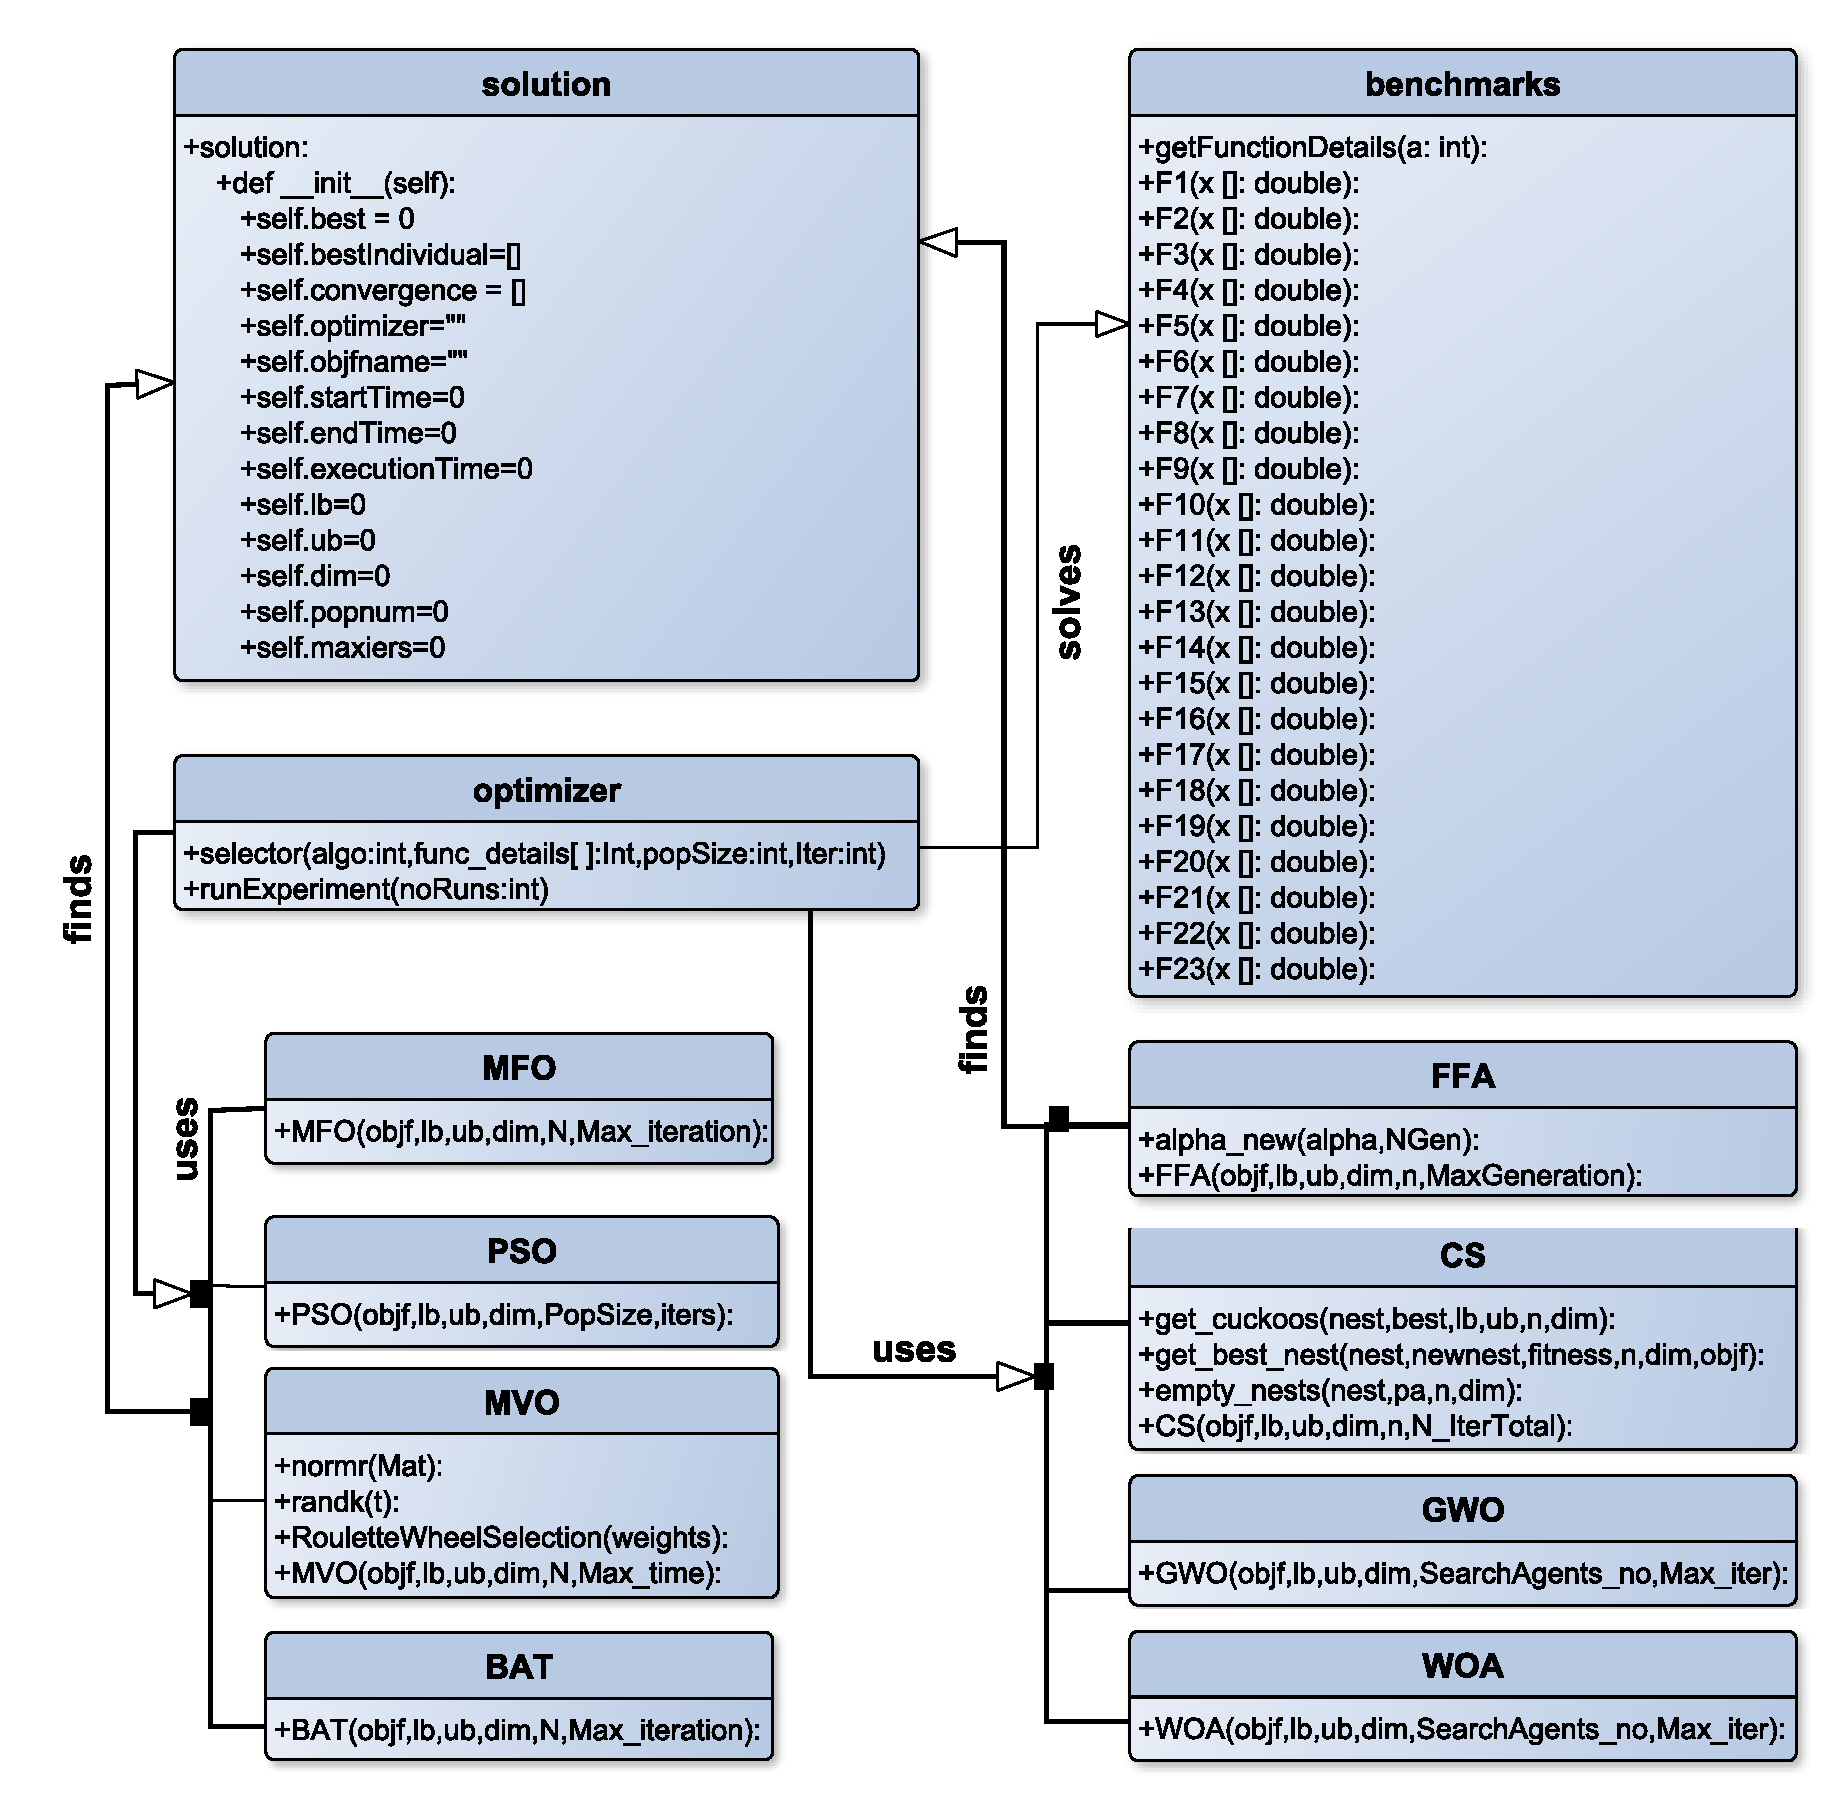
\includegraphics[scale=0.52]{classD.eps}}
\caption{Class diagram of the EvoloPy framework}
\label{fig:framework}
\end{figure*}

We use the UML representation to demonstrate the main components of EvoloPy framework. A class diagram illustrating the EvoloPy components and their relationships is presented in Figure \ref{fig:framework}. The EvoloPy framework consists of eleven classes, three of them for coordinating and simplifying the optimization process, namely; optimizer, benchmarks, and solution. On the other hand, the other eight classes representing the actual nature-inspired optimizers. The core flow of EvoloPy relies in that an optimizer solves a benchmark using one or more optimizers to find global solutions. We have used a generic classes names in the framework in order to make it very easy to flow and general enough to be modified and usable.





\section{\uppercase{Comparison with Matlab}}

In this section we compare the metaheuristic algorithms implemented so far in EvoloPy with their peers in Matlab based on their running time. The idea here is to measure the running time of the main loop of each algorithm in EvoloPy and Matlab with an equal number of function evaluations. The experiments were performed on on a personal machine with an  Intel(R) Core(TM) i5-2400 CPU at 3.10Ghz and a memory of 4 GB running Windows 7 professional 32bit operating system. In all experiments, the population size and the number of iterations was set for all algorithms to 50, and 100, respectively. In order to study the effect of the size of the problem to be solved on the running time of the algorithms, all optimizer were executed using different dimension lengths ranging from a small number of 50 elements reaching up to 20,000 in both implementations, Matlab and EvoloPy. Note that the dimension length here indicates number of elements in the single individual or in another words, number of of variables in the objective function. All optimizers were applied to minimize the unimodal function given in Equation \ref{eq:f3}. 



\begin{equation}
f(x)=\sum_{i=0}^{n-1}(\sum_{j=0}^{i-1}x_{j})^{2}
\label{eq:f3}
\end{equation}

The results of EvoloPy and Matlab implementations are shown in Figure \ref{fig:comparison-time}. It can be noticed that with small dimension sizes there is no big significant difference in the running time between the two implementations. In most of the optimizers and up to a dimension size of 500  the running time was less than 250 second. However, for higher sizes, the difference in the running time  remarkably increases. On a dimension length of 20,000 the ration was around 1:2 for most of the optimizers.

The efficient running time of EvoloPy compared to Matlab implementation when applied for solving problems with large number of variables can be explained due to the use of the powerful N-dimensional array object \texttt{NumPY} to represent individuals and populations.

\begin{figure*}[H]
\centering
\begin{tabular}{ c c  }
\centering
\subfigure[BAT]{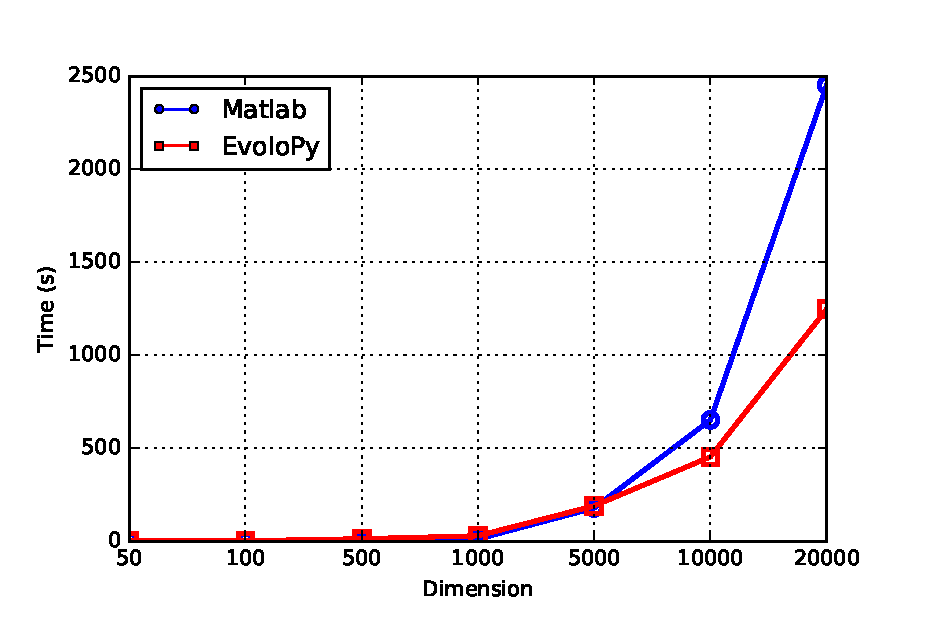
\includegraphics[scale=.45]{BAT.eps}\label{t1}} & 
\subfigure[CS]{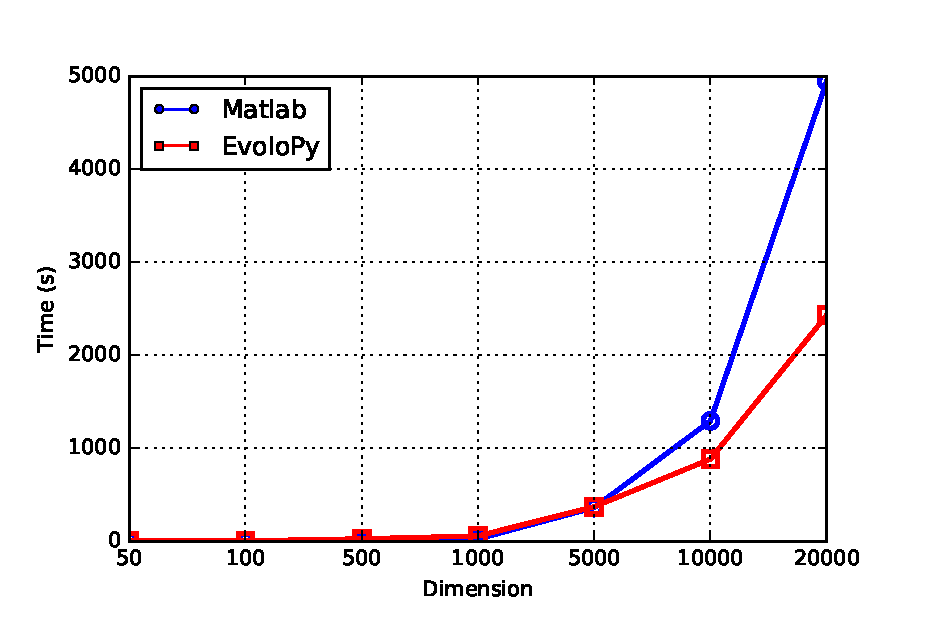
\includegraphics[scale=.45]{CS.eps}} 


\\
\subfigure[FFA]{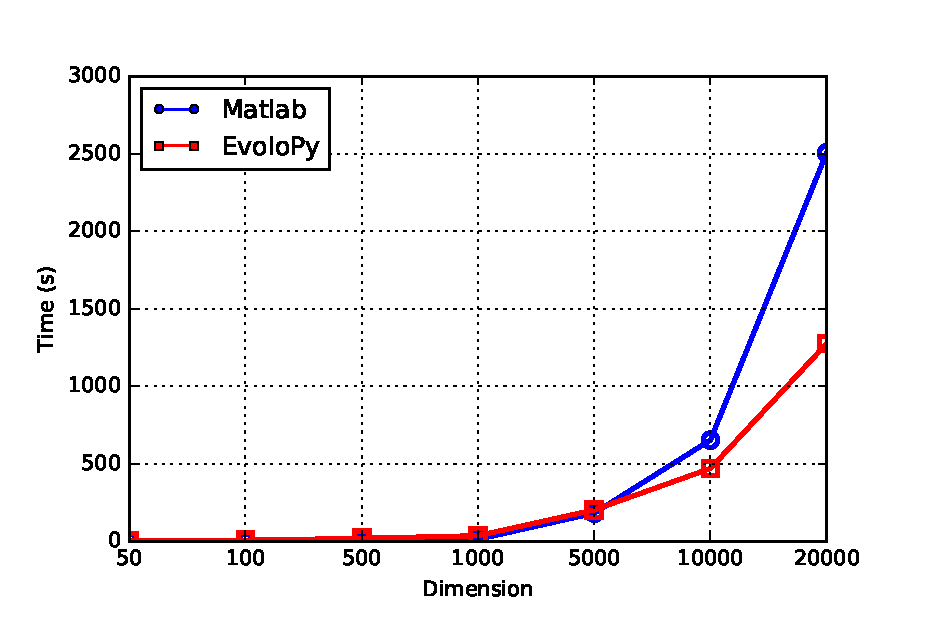
\includegraphics[scale=.45]{FPA}\label{subfigf6t}} & 
\subfigure[GWO]{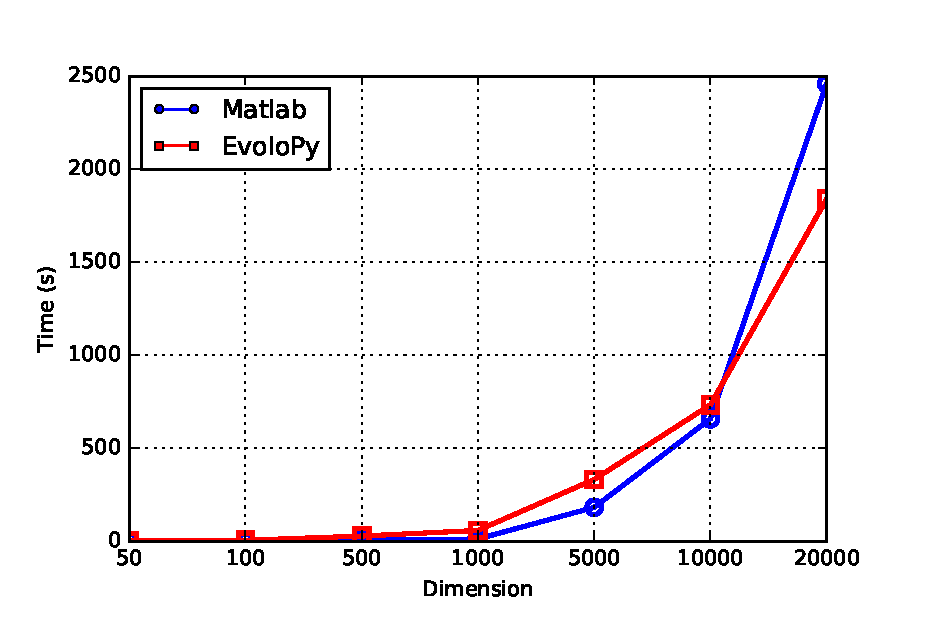
\includegraphics[scale=.45]{GWO}\label{subfigf2s}} 


\\
\subfigure[MFO]{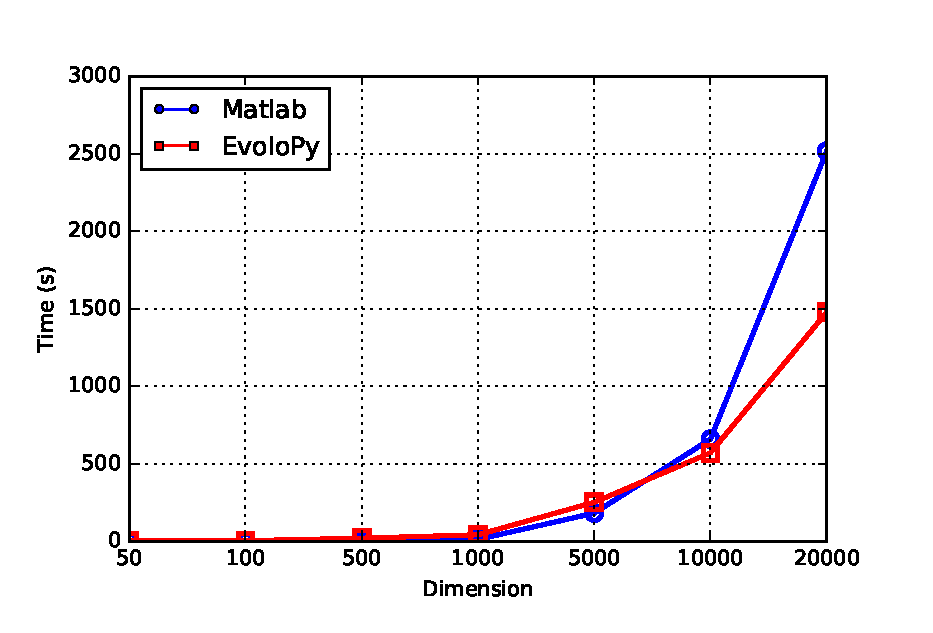
\includegraphics[scale=.45]{MFO.eps}\label{subfigf4s}} & 
\subfigure[MVO]{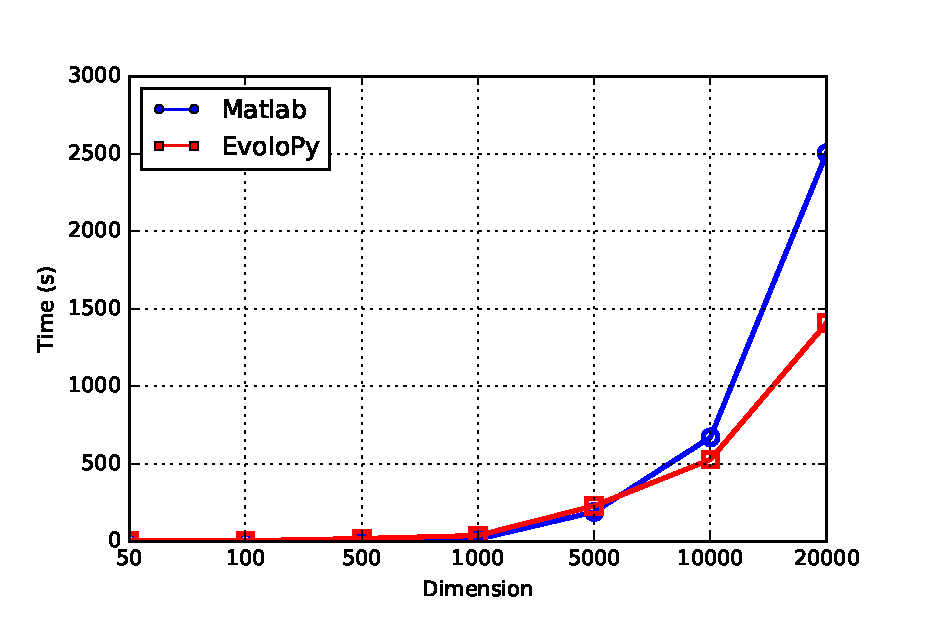
\includegraphics[scale=.45]{MVO.eps}\label{subfigf6s}}

\\

\subfigure[PSO]{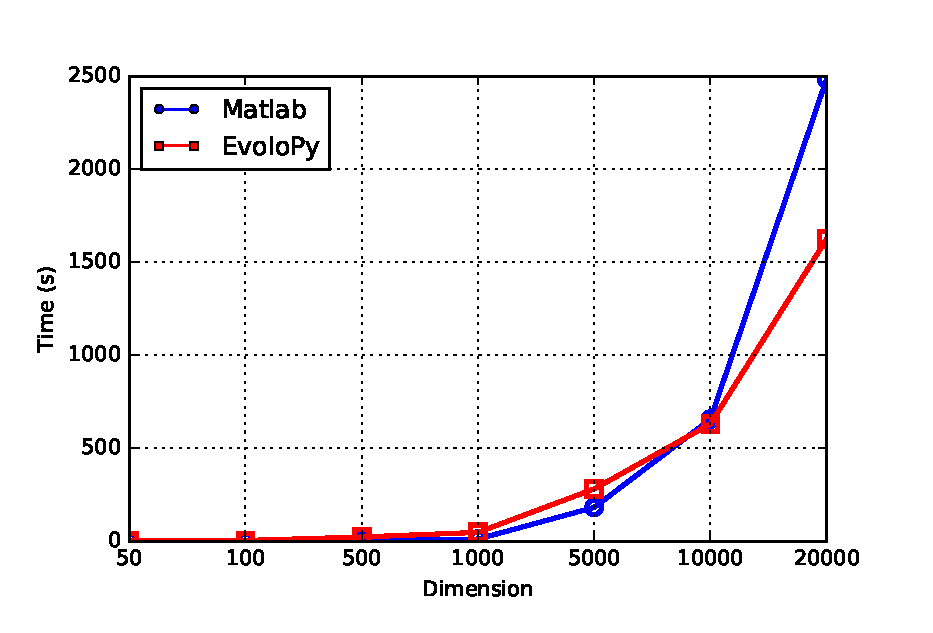
\includegraphics[scale=0.45]{PSO.eps}\label{t2}} &  
\subfigure[WOA]{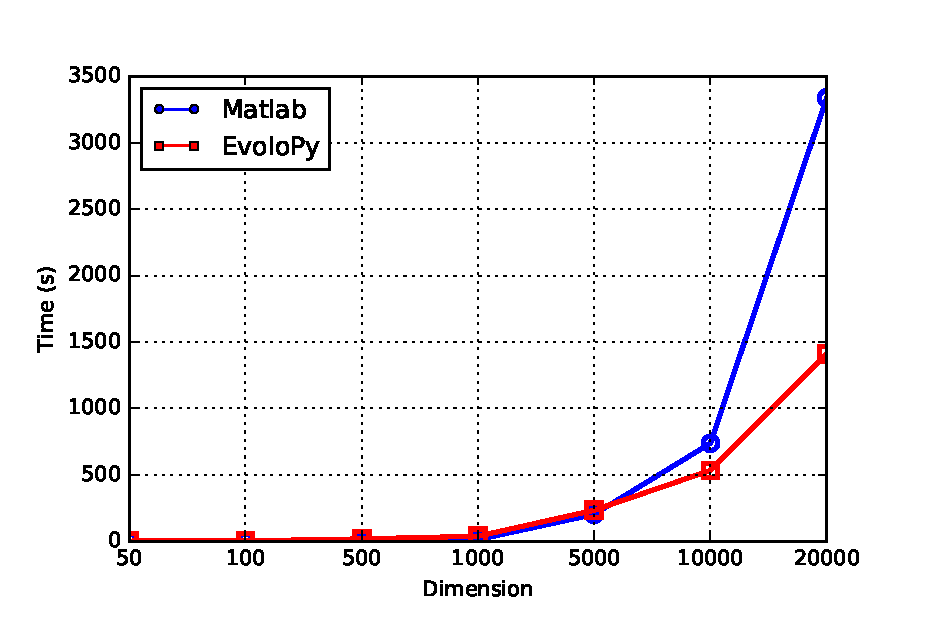
\includegraphics[scale=0.45]{WOA.eps}\label{subfigf4t}} 


\\

\end{tabular}

\caption{Comparison between between the metaheuristic optimizers in EvoloPy and Matlab based on execution time of the main iteration.}
\label{fig:comparison-time}
\vspace{-0.0in}
\end{figure*}






%\subfigure[Liver]{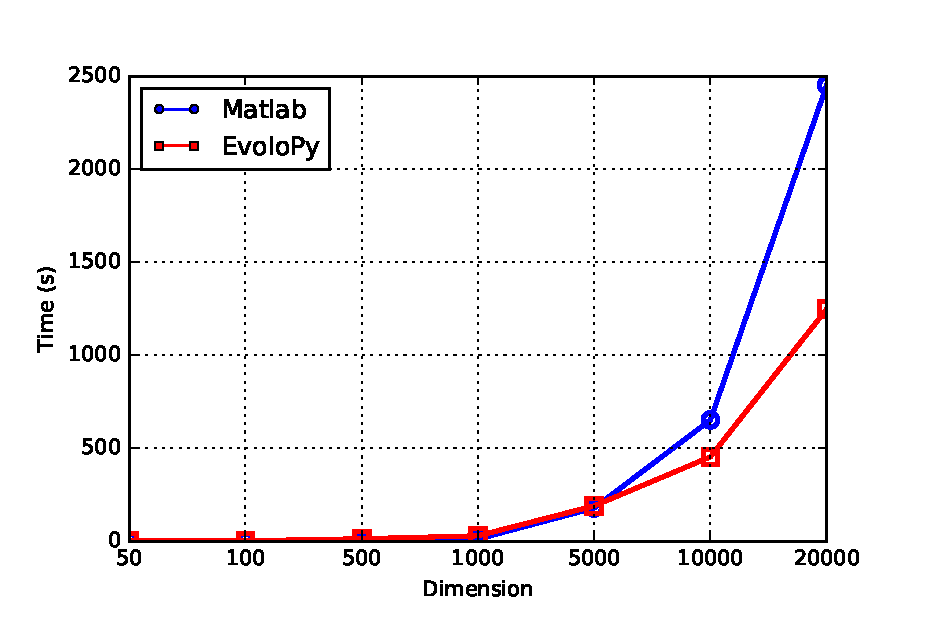
\includegraphics[scale=0.35]{BAT.eps}\label{subfigf6t}} 

\section{\uppercase{Conclusions and future work}}




\vfill
\bibliographystyle{apalike}
{\small
\bibliography{ref}}



\end{document}

